% !TeX root = ../Main-Report.tex

\chapter{Task Space Motion}
This section document the implementation of movements in task space. 

\section{Trapezoidal trajectory in task space}

The same waypoints from the joint space motion have been used, which are visible in table \ref{tab:jspace_waypoints}. The maximum velocity of the end-effector was set to be $0.04\,\si{\meter\per\second}$, the maximum acceleration $0.07\,\si{\meter\per\square\second}$. The motion of the end-effector can be viewed in figure \ref{fig:tspace_trapz_traj}.

\begin{figure}[H]
	\centering
	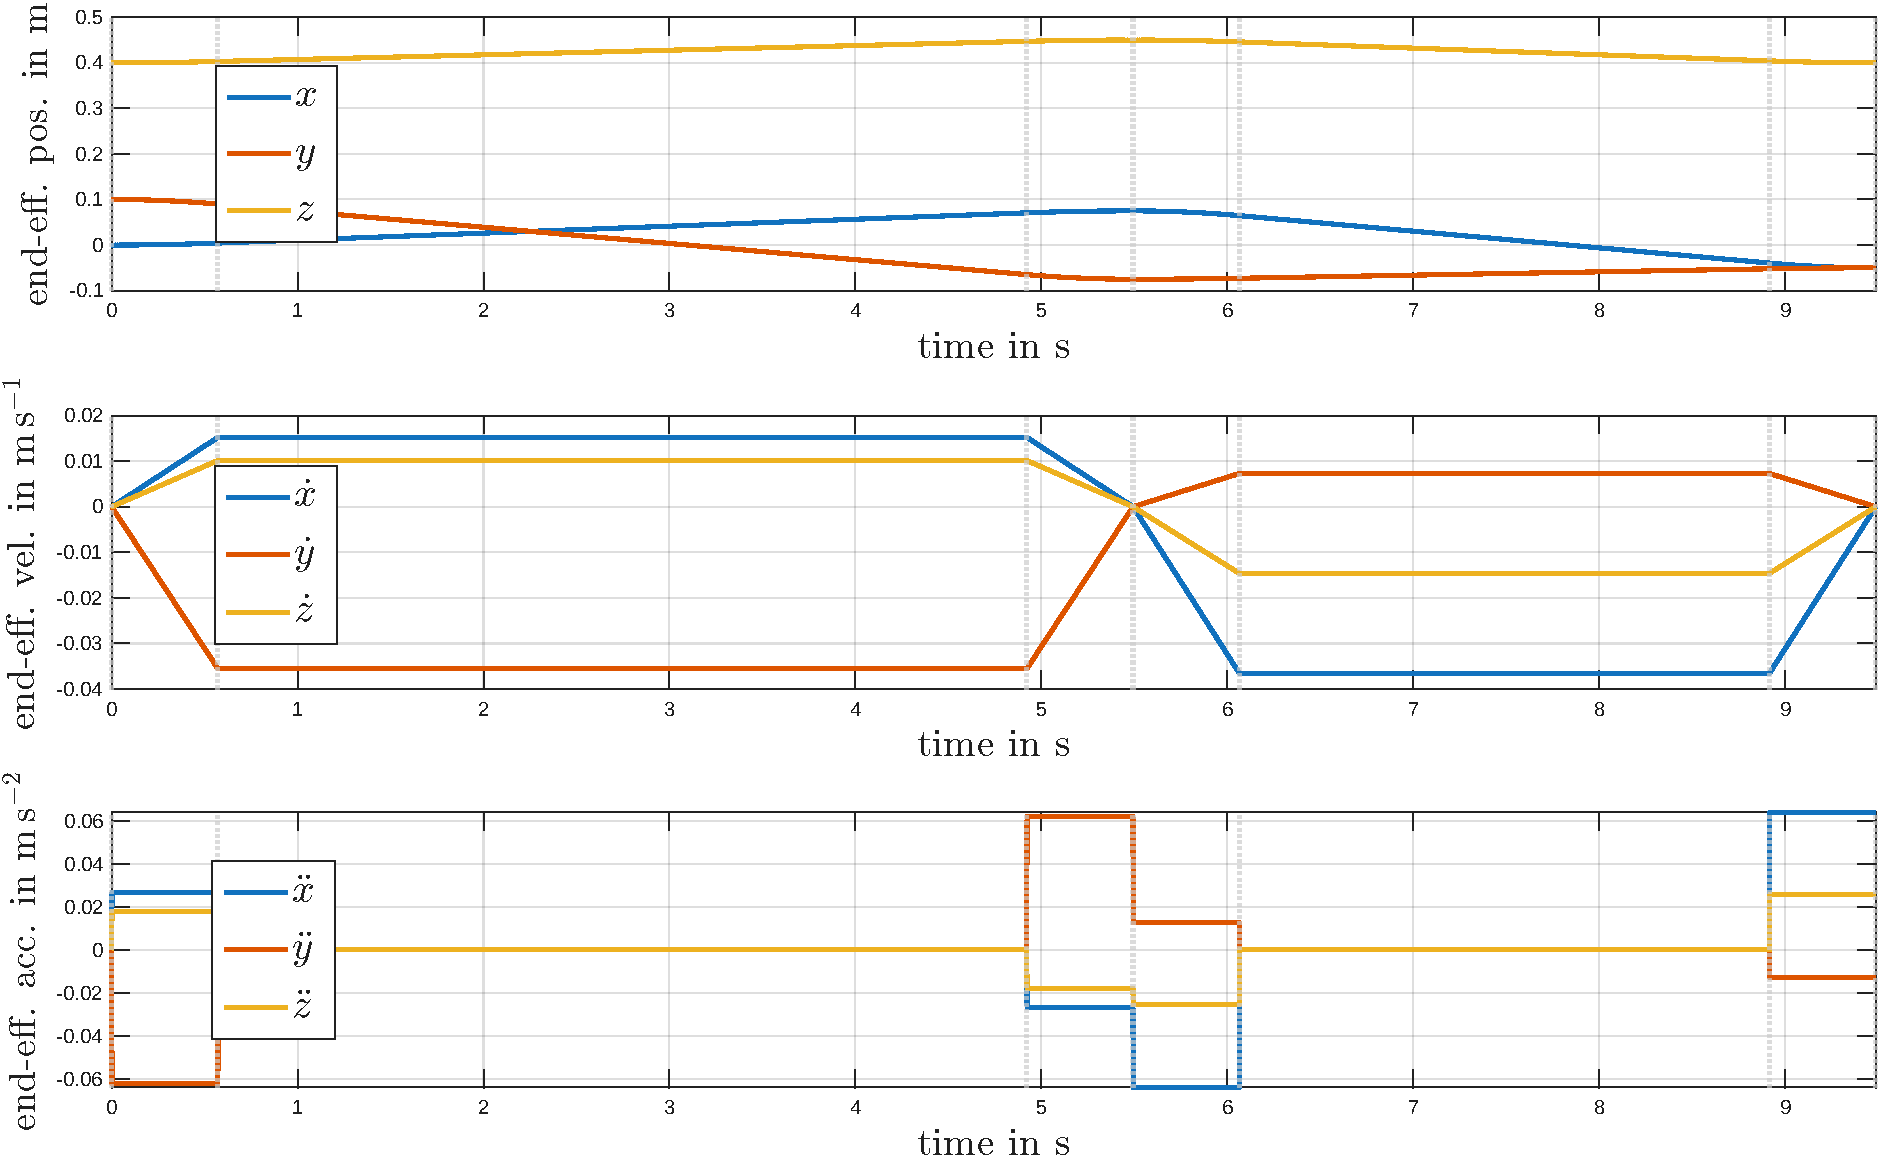
\includegraphics[width=1.0\linewidth]{cus_imgs/task_trapz.pdf}
	\caption{Position, velocity and acceleration of the end-effector for task space motion}
	\label{fig:tspace_trapz_traj}
\end{figure}

As expected, the end-effector moves in a straight line from point to point. The acceleration and velocity constraints are fulfilled.

\section{Double-S trajectory in task space}
Similar to the double-S velocity profile in task space, using a trapezoidal acceleration profile for task space trajectories make it possible to limit the jerk. In this case, the maximum jerk was set to $5\,\si{\meter\per\cubic\second}$.

\begin{figure}[H]
	\centering
	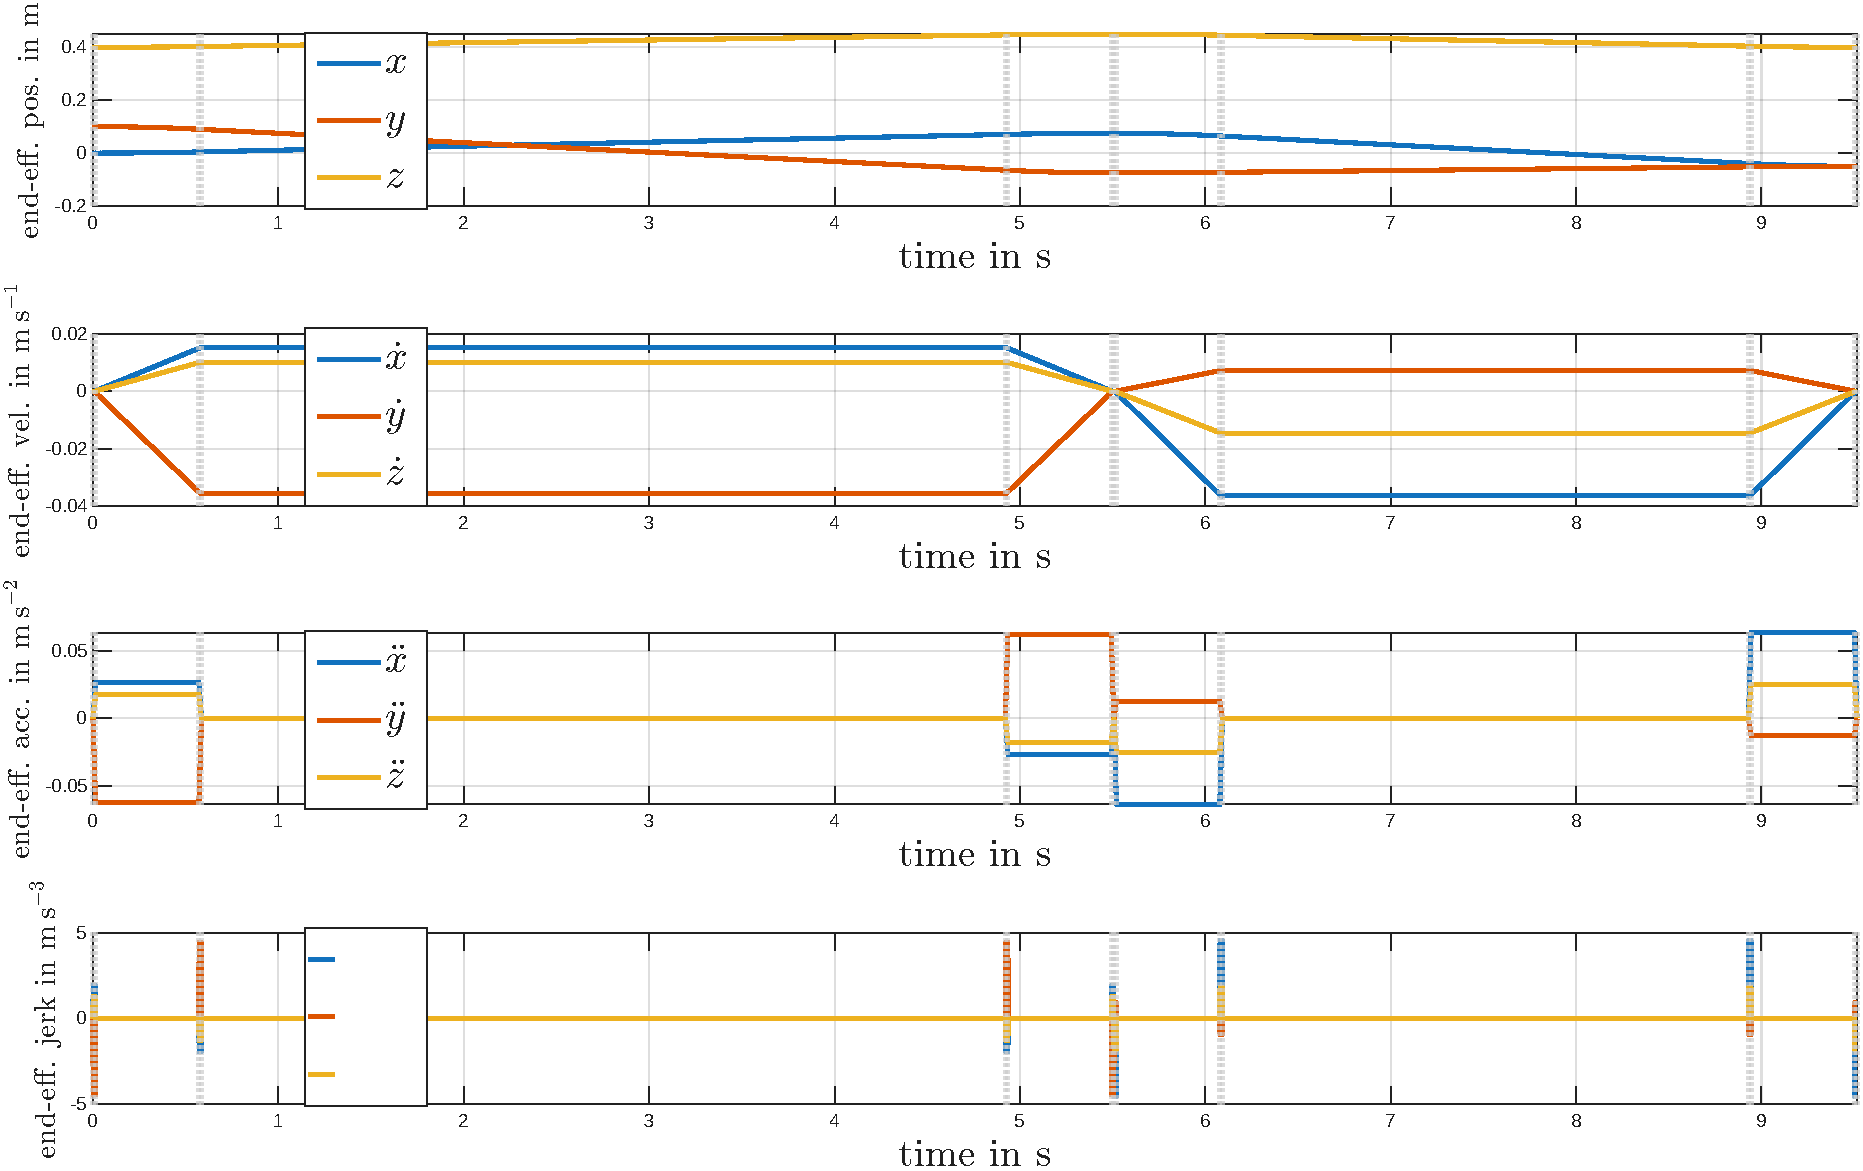
\includegraphics[width=1.0\linewidth]{cus_imgs/task_double_s.pdf}
	\caption{Double-S trajectory, including position, velocity, acceleration and jerk profiles in task space}
	\label{fig:tspace_ds_traj}
\end{figure}

As the jerk limit is relatively high, the double-S shape of the velocity of the end-effector is barely visible, but it is still there.


\section{Comparison joint and task space} \label{sec:comparison_jspace_tspace}

Compared to the joint space motion, the task space motion takes more time to execute within the constraints. A comparison of the joint velocities and accelerations for the trapezoidal velocity profiles for both can be viewed in figure \ref{fig:jspace_vs_tspace}.

\begin{figure}[H]
	\centering
	
\includegraphics[width=1.0\linewidth]{cus_imgs/joint_vs_task.pdf}
	\caption{Velocity and acceleration of the joints for joint and task space motion (trapezoidal)}
	\label{fig:jspace_vs_tspace}
\end{figure}

It is apparent that the joint velocities and accelerations in task space (right column) are much smaller than in joint space (left column). This is the cause of the motion taking significantly longer. The difference in the path that the end-effector takes in both motion modes can be viewed in figure \ref{fig:jspace_vs_tspace_motion}.

\begin{figure}[H]
	\centering
	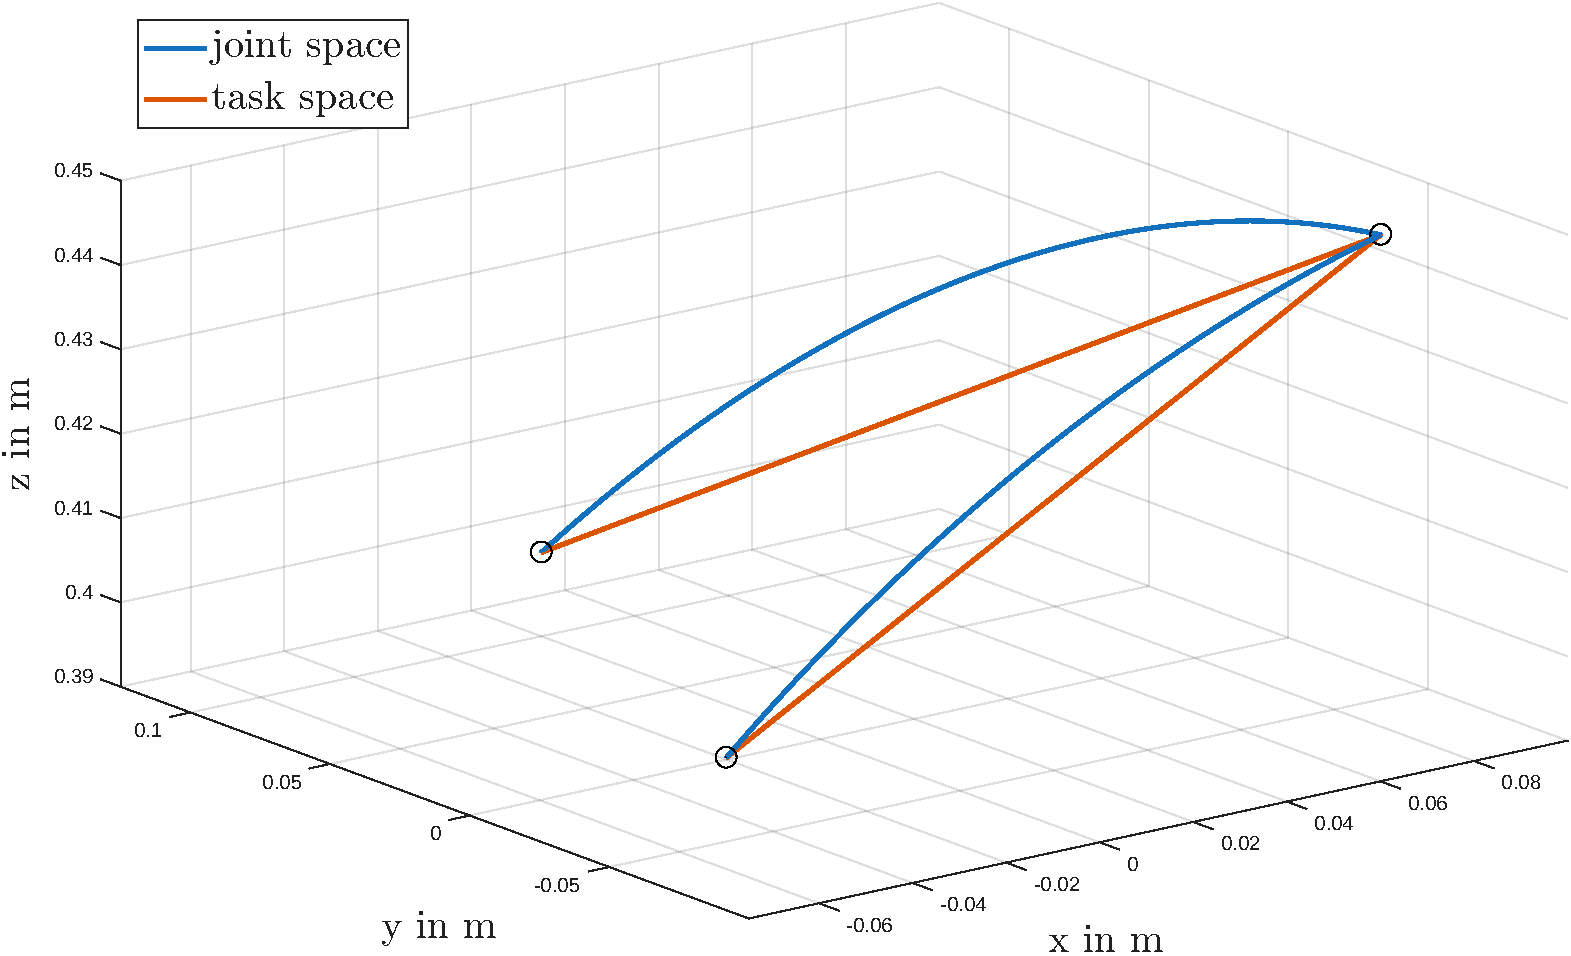
\includegraphics[width=0.9\linewidth]{cus_imgs/joint_vs_task_motion_3d.pdf}
	\caption{End-effector position in joint and task space}
	\label{fig:jspace_vs_tspace_motion}
\end{figure}

The Simulink setup used to fullfill these tasks (and parts of the next) can be seen in figure \ref{fig:joint_task_simulink}.

\begin{figure}[H]
	\centering
	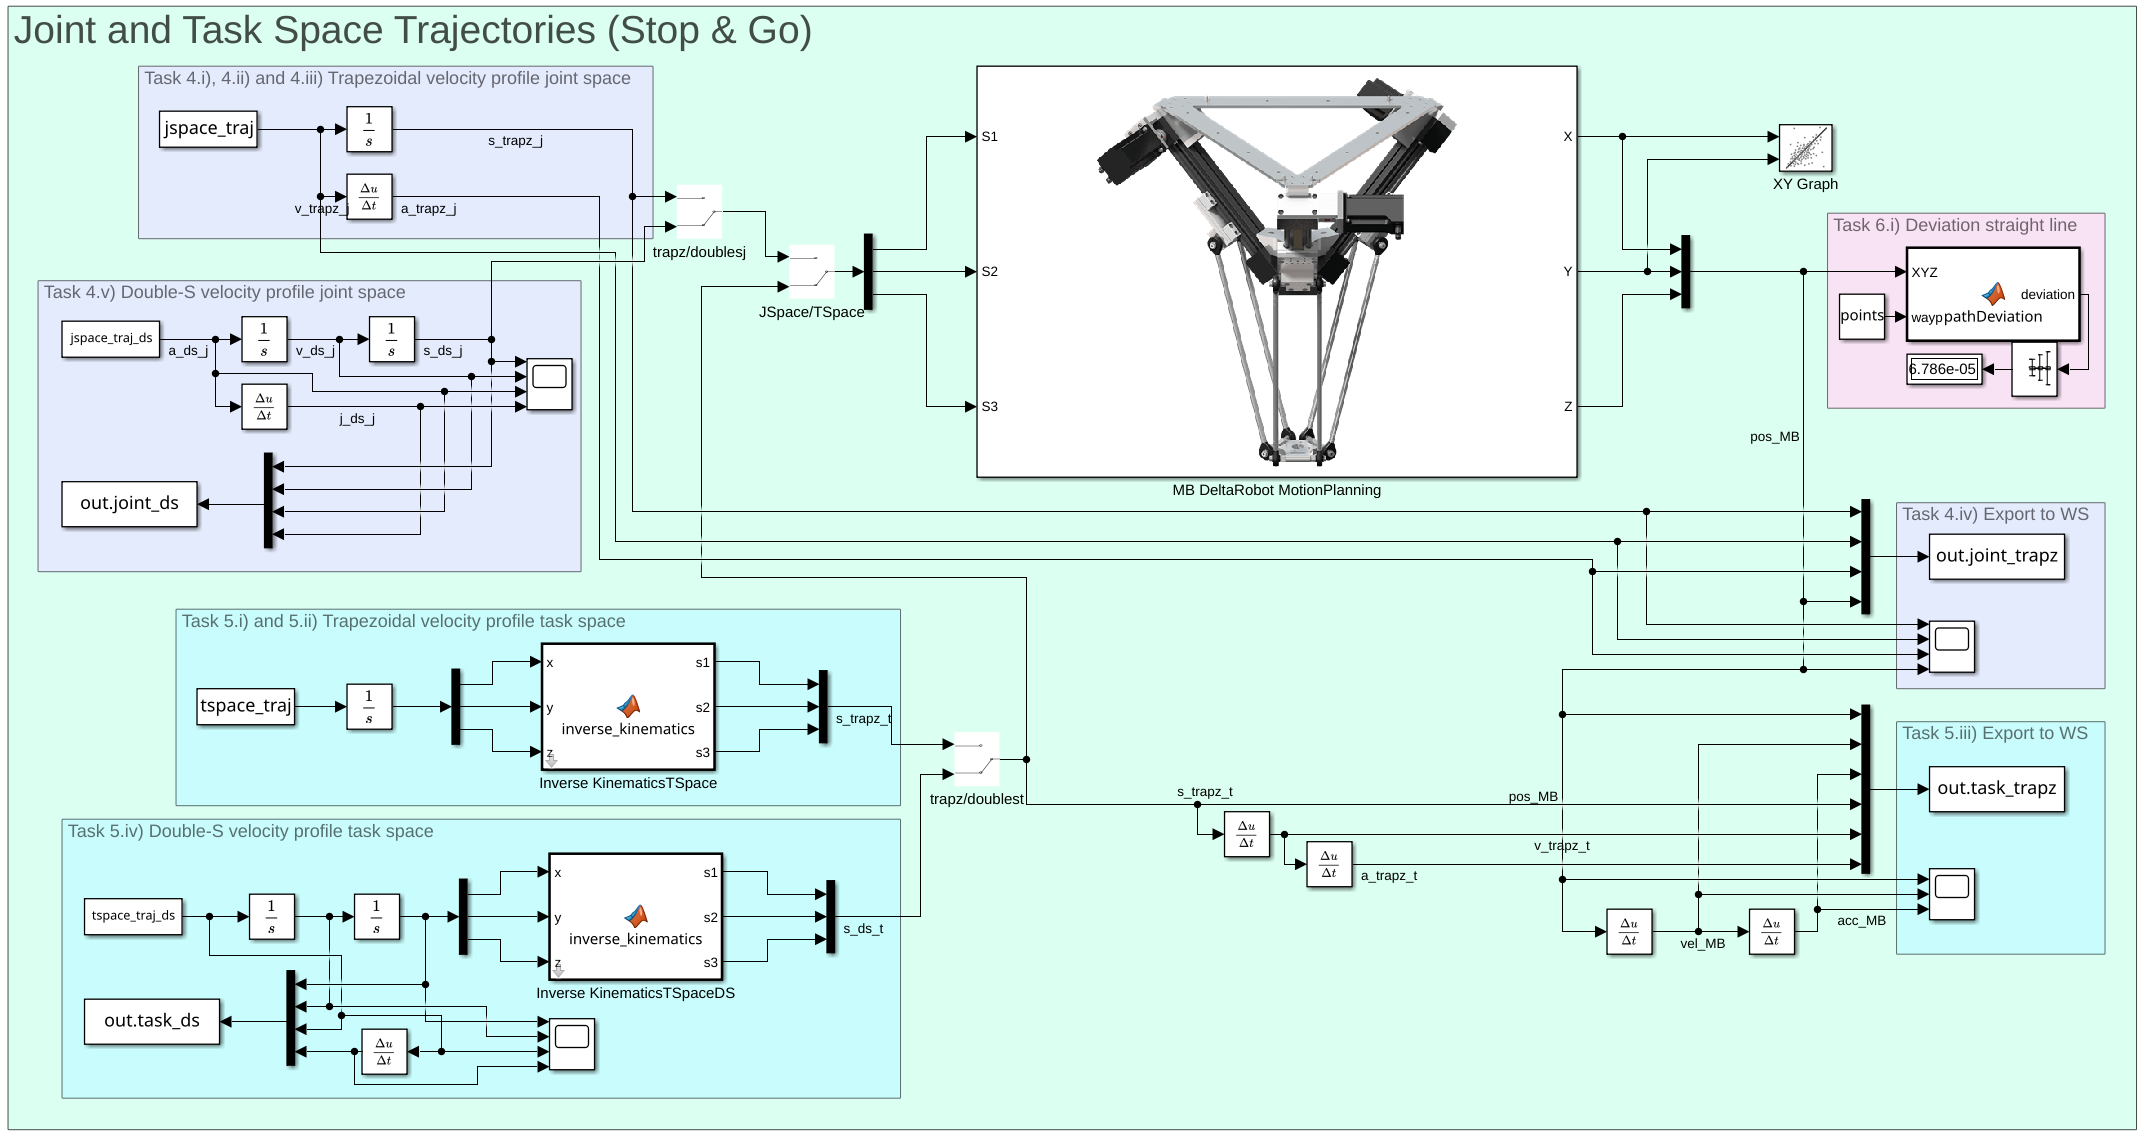
\includegraphics[width=1.0\linewidth]{cus_imgs/JSPACE_TSPACE_simulink.png}
	\caption{Simulink layout for joint and task space trajectories}
	\label{fig:joint_task_simulink}
\end{figure}